
\chapter{Hilbert Schemes}
\label{HilbertSchemesChapter}

In earlier chapters, we described some  degree $d$ embeddings of curves
of  genus $g$ in projective spaces $\PP^r$ for small $g,r,d$. In this
chapter, we will try to describe the \emph{restricted Hilbert scheme}
\index{restricted Hilbert scheme}%
\index{Hilbert scheme!restricted}%
\index{Hilbert scheme|(}%
$\cH^\circ_{g,3,d}$, defined to be the open subscheme of the Hilbert
scheme $\cH_{g,3,d} \colonequals  \Hilb_{dm-g+1}(\PP^3)$ parametrizing smooth,
\index{H .,3,d@$\cH_{g,3,d}$}%
\index{Hilb@$\Hilb_{dm-g+1}$}%
irreducible and nondegenerate curves of degree $d$ and genus $g$
in $\PP^3` `$.

Three basic questions about the schemes $\cH^\circ_{g,r,d}$ are:

\begin{enumerate}
\item[$\bullet$] Is $\cH^\circ_{g,r,d}$ irreducible?
\item[$\bullet$]  What is its dimension (or the dimensions of its
components)?
\item[$\bullet$] Where is it smooth, and where is it singular?
\end{enumerate}

Of course, there are many more questions one could ask about the geometry
of $\cH^\circ_{g,r,d}$, many of which are open. For example,  what is the
closure $\overline{\cH^\circ_{g,r,d}} \subset \cH_{g,r,d}$ in the whole
Hilbert scheme? (In other words, when is a subscheme $X \subset \PP^r$
with Hilbert polynomial $dm-g+1$ \emph{smoothable}, in the sense that it
\index{smoothable}%
is the flat limit of a family of smooth curves?) In general, no one knows!


\section{Degree 3}\label{degree 3}

The first case to consider is that of the Hilbert scheme
$\cH_{0,3,3}$. The corresponding restricted Hilbert scheme
\index{restricted Hilbert scheme}%
$\cH^\circ_{0,3,3}$, parametrizing
twisted cubics,
\index{twisted cubic}%
is one we have
encountered and described already: in Proposition~\ref{hilb of twisted
cubics} we showed that $\cH^\circ_{0,3,3}$ is irreducible of dimension 12,
\index{H 0,3,3@$\cH_{0,3,3}$, second component of}%
and we gave another proof, based on linkage, in
Chapter~\ref{LinkageChapter}.
By Exercise~\ref{twisted cubic normal bundle}, the normal bundle of a
\index{normal!bundle}%
twisted cubic $C$ is $\sN_{C/\PP^3}=\sO_{\PP^1}(5)\oplus \sO_{\PP^1}(5)$
so by Theorem~\ref{tangent space of Hilb} the tangent space to the
Hilbert scheme at $C$ is
$H^0(\sN_{C/\PP^3}) = \CC^{12}$. Thus $\cH_{0,3,3}$ is smooth at this
point.

\subsection*{The other component of
\texorpdfstring{$\cH_{0,3,3}$}{$H_{0,3,3}$}}

\hskip-2.5pt
We might expect that the closure $\overline{\cH^\circ_{``0,3,3}}$
would be all of $\cH_{0,3,3}$, but this is not the case:  $\cH_{0,3,3}$
has two irreducible components.

\hskip-0.5pt
One component is the closure of $\cH^\circ_{``0,3,3}$. 
\hskip-1pt To describe the \kern-0.3pt ``extraneous'' \kern-0.3pt 
second component, suppose we start with a plane cubic
curve $C_0 \subset \PP^2 \subset \PP^3` `$. This is of course a curve of
degree 3, but its Hilbert polynomial is $p(m) = 3m$ rather than $3m+1$,
reflecting the fact that the genus of $C_0$ is 1, not 0.

But that can be fixed: adding a point $p \in \PP^3 \setminus C_0$
to $C_0$ has the effect of increasing the Hilbert polynomial by 1, so
that the Hilbert polynomial of $C \colonequals  C_0\cup \{p\}$ is $3m+1$. Thus
$C$  corresponds to a point of $\cH_{0,3,3}$. In fact, the locus
in $\cH_{0,3,3}$ of curves $C$ of this form is open, and its closure
$\cH'$, which includes plane cubics with an embedded point, is a second
irreducible component of $\cH_{0,3,3}$.


\begin{theorem}
$\cH_{0,3,3}$ has two irreducible components
{\normalfont(Figure~\ref{Fig18.1})}. One
has generic point corresponding to  a twisted cubic,
and the other has generic point corresponding to the union of a smooth
plane cubic and a point outside the plane.
They have
dimensions
\1\2 and \1\5 respectively.
\end{theorem}

\begin{proof}
Let $C'$ be the purely 1-dimensional scheme defined by the intersection
of the 1-dimensional primary ideals in the decomposition of $I_C$. If
the Hilbert polynomials of $C$ and $C'$ are $p(m)$ and  $p'(m)$ then
$p(m) \geq p'(m)$ for all large $m$; equality for large $m$ would imply
that $C'=C$.

Whatever 0-dimensional components $C'$ may have do not contribute
to the degree (= leading coefficient of the Hilbert polynomial) so
$\deg C' = \deg C = 3$. Thus the curve $C'$ is either irreducible or
the union of two or three irreducible components. In the first case
$C'$ is either nondegenerate, in which case it is a twisted cubic
by Theorem~\ref{characterization of P1} and $C' = C$; or a plane
cubic. If $C'$ is a plane cubic, then it has Hilbert function $3m$,
so $\sI_{C'}/\sI_C$
corresponds to a point in $\PP^3` `$, either embedded in $C'$ or not. Such
a union is specified by the choice of the
plane, the cubic in it, and the point,%
\footnote{If the point is an
embedded point, specifying $C'$ and $p$ does not determine $C$\emdash if $p$
is a smooth point of $C'$, for example, there is a one-parameter family
of curves $C$ with support $C'$ and an embedded point at $p$; the tangent
space to $C$ at $p$ can be any plane containing the tangent line to $C'$
at $p$\emdash but these are all flat limits of disjoint unions $C' \sqcup
\{p\}$, so they don't contribute a separate component of $\cH_{0,3,3}$.}
and thus has dimension $3+9+3 = 15$.

On the other hand, if $C$ is not planar and not irreducible, then $C'$
consists of 3 lines or the union of a (planar) conic
and a line not in the plane. In this case each connected component has
arithmetic genus 0 and thus Hilbert polynomial
with constant term 1; so the curve must be connected. All such curves
can be realized as divisors of type $(1,2)$
on a quadric, and thus have Hilbert function equal to that of $C$,
whence again $C' = C$.
\end{proof}

\begin{figure}
\leavevmode
\vskip-0.05in\leavevmode
\raise7pt\hbox{
\includegraphics[width=1.2in]{main/Fig18-1A-new}}\quad
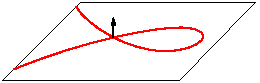
\includegraphics[width=1.7in]{main/Fig18-1B-new}%
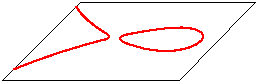
\includegraphics[width=1.7in]{main/Fig18-1C-new}%
\hskip-20pt\raise0.6in\hbox{\Large{\color{red}$\cdot$}}\hskip20pt%

\centerline{\small$\in \sH^\circ_{0,3,3}$\hfil\hfil 
$\in \sH^\circ_{0,3,3}\cap \sH'_{0,3,3}$\hfil\hfil 
\quad$\in \sH'_{0,3,3}$\qquad}

\caption{$\sH_{0,3,3}$ has two components, whose generic members are
shown on the left and right,
with the generic member of the intersection shown in the middle. On
the left is
a generic point of the ``principal'' component: a
smooth
twisted cubic. This degenerates to a singular plane
cubic with an embedded point at the node. In the other component, the
singular plane cubic
becomes smooth, and the extra point is free to move anywhere in space.}
\label{Fig18.1}
\end{figure}

\begin{fact}
In \cite{Piene-Schlessinger} it is also shown that the two components
\index{Piene @Piene, Ragni}%
\index{Schlessinger @Schlessinger, Michael}%
of $\cH_{0,3,3}$ are smooth and rational and that
their  intersection is  smooth and rational of dimension 11.
\end{fact}

The presence of components of the Hilbert scheme whose general member is
not smooth, irreducible and nondegenerate is not exceptional, and in the
following section we'll describe some of the ``extraneous'' components more
generally. But one aspect of the geometry of $\cH_{0,3,3}$ is special:
the action of the group 
$\PGL_4$
\index{PGL@$\PGL_4$}%
on $\cH_{0,3,3}$ has only finitely
many orbits (if you want to see the orbits in the
principal
component
$\overline{\cH^\circ_{0,3,3}}$, see \cite{Montreal}). It's not known if
there are other examples of this, beyond Grassmannians, Hilbert schemes
of quadric hypersurfaces and Hilbert schemes of triples of points.
Later (page~\pageref{rigid?})
we will discuss the opposite situation: the
\index{rigid curve}%
possibility of ``rigid curves,''  corresponding to points in the Hilbert
\index{Hilb@$\Hilb_{dm-g+1}$}%
scheme $\cH^{\circ}_{dm-g+1}$ with $g>0$ whose $\PGL_{r+1}$ orbit is open.

\section{Extraneous components}

Let $\cH_d(\PP^r)$ be the Hilbert scheme of subschemes of $\PP^r$
with Hilbert polynomial of degree 0, say equal to the constant $d$.
There is an open subset $\cH^\circ_d(\PP^r)$ of dimension $dr$ whose
points correspond to reduced $d$-tuples of points in $\PP^r` `$. This
open subset is isomorphic to the complement of the diagonals in the
$d$-th symmetric power of $\PP^r` `$. We call the closure of this open
set the \emph{principal component} of $\cH_d(\PP^r)$.
\index{principal component}%

The Hilbert scheme  $\cH_d(\PP^2)$ is smooth and irreducible of dimension
$2d$, and a similar result holds for
0-dimensional schemes on any smooth surface, but Iarrobino
\citeyear{Iarrobino1985}
\index{Iarrobino, Anthony A., Jr.}%
showed
that, for any $r \geq 3$ and any sufficiently large $d$, there are
components of $\cH_d(\PP^r)$ having dimension strictly larger than $dr$;
\index{H d@$\cH_d(\PP^r)$}%
see Exercise~\ref{bigger component}. There are
also examples of extraneous components
\index{extraneous components}%
of dimension $<dr$; see \cite{MR2579394}. No one knows how many
irreducible components the Hilbert scheme $\cH = \cH_d(\PP^r)$ has,
or what their dimensions might be.

This in turn infects the Hilbert schemes of curves. For example,
the Hilbert scheme $\cH_{g,r,d}$ has a component whose general point
\index{H .,3,d@$\cH_{g,3,d}$}%
corresponds to a union of a plane curve of degree $d$ and $\tbinom{d-1}{2}
- g$ points; moreover, if $\Gamma$ is any irreducible component of the
Hilbert scheme of zero-dimensional subschemes of degree $\tbinom{d-1}{2} -
g$ in $\PP^3` `$, there is a component of $\cH_{g,3,d}$ whose  general point
corresponds to a union of a plane curve of degree $d$ and the subscheme
corresponding to a general point of $\Gamma$. Further, we can replace the
plane curves in this construction with any component of the Hilbert scheme
of curves of degree $d$ and genus $g'>\nobreak g$. There can also be components
of $\cH_{g,3,d}$ whose general point corresponds to a subscheme of $\PP^3$
with a spatial embedded point\emdash see \cite{Chen-Nollet}.

Bottom line: it's a mess. For many $g,d$ the Hilbert scheme $\cH_{g,3,d}$
has many components. In most cases no one knows how many, or what their
dimensions are, which is why we most often focus on the restricted
Hilbert scheme.

\section{Degree 4}\label{degree 4 genus 0}

By Clifford's theorem, an irreducible nondegenerate curve of degree 4
in $\PP^{3}$ must have genus 0 or 1; we consider these cases in turn.

\subsection*{Genus 0}

We can deal with
rational quartics
\index{rational!quartic}%
by a slight variant of the first method
we used to deal with twisted cubics. A rational curve of degree 4 is the
image of a map $\phi_F : \PP^1 \to \PP^3$ given by a four-tuple $F =
(F_0,F_1,F_2,F_3)$ with $F_i \in H^0(\cO_{\PP^1}(4))$. The space of
all such four-tuples up to scalars is a projective space of dimension
$4 \times 5 - 1 = 19$; let $U \subset \PP^{19}$ be the open subset of
four-tuples such that the map $\phi$ is a nondegenerate embedding. By the
universal property of the Hilbert scheme there is a surjective map $\pi :
U \to \cH^\circ_{0,3,4}$, whose fiber over a point $C$ is the space of
\index{H 0,3,4@$\cH_{0,3,4}$}%
maps with image $C$. Since any two such maps differ by an automorphism
\index{PGL@$\PGL_2$}%
of $\PP^1$\emdash that is, an element of 
$\PGL_2$
\emdash the fibers of $\pi$ are
three-dimensional, proving that $\cH^\circ_{0,3,4}$ is irreducible of
dimension 16.

The same analysis can be used on rational curves of any degree $d$
in any projective space $\PP^r$:

\begin{proposition}\label{dimension of rational curves}
The open set $\cH^\circ_{0,r,d}$ parametrizing smooth, irreducible
\index{H 0, ,d@$\cH_{0,r,d}$}%
non\-degenerate rational curves $C \subset \PP^r$ is irreducible of
dimension $(r+1)(d+1)-4$; in~case $r=3$ in particular it has dimension
$4d$.
\end{proposition}

\begin{proof}
The space $U$ of nondegenerate embeddings $\PP^1 \to \PP^r$ of degree
$d$ is an open subset of the projective space $\PP^{(r+1)(d+1)-1}$ of
$(r+1)$-tuples of homogeneous polynomials of degree $d$ on $\PP^1$ modulo
scalars; and the fibers of the corresponding map $U \to \cH^\circ_{0,r,d}$
\index{PGL@$\PGL_2$}%
are copies of 
$\PGL_2$.
\end{proof}

In contrast to the case of twisted cubics, smooth rational curves in
$\PP^r$ of the same degree may have different normal bundles. This gives
an interesting stratification of the restricted Hilbert scheme of rational
\index{Coskun@Co\c{s}kun, \.{I}zzet}%
\index{Riedl @Riedl, Eric}%
curves; see \cite{MR3778979} for a discussion.

\subsection*{Genus 1}
 As we saw in Section~\ref{g=1 in P3}, a quartic curve $C \subset \PP^3$
 of genus 1 is the intersection of two quadric surfaces, and by Lasker's
\index{Lasker's theorem}%
 theorem, every quadric containing $C$ is a linear combination of those
 two. Conversely, the intersection of two general quadrics in $\PP^3$ is
 a quartic curve of genus 1, as follows from B\'ezout's theorem
\index{Bezout@B\'ezout's theorem}%
and the
 adjunction formula. We
\index{adjunction formula}%
can thus construct a family of quartics of genus
 1: let $V = H^0(\cO_{\PP^3}(2))$ be the 10-dimensional vector space of
 homogeneous quadric polynomials in $\PP^3$ and $G(2,V)$ the
Grassmannian of 2-planes
\index{G@$G(2,V)$}%
in $V` `$, and consider the
incidence correspondence
\index{incidence correspondence}%
$$
\Gamma = \bigl\{@(\Lambda, p) \in G(2,V) \times \PP^3 \mid F(p)=0 \; \forall \;
F \in \Lambda@\bigr\}.
$$
The fiber of $\Gamma$ over a point $\Lambda \in G(2,V)$ is thus the
base locus of the pencil of quadrics represented by $\Lambda$; let $B
\subset G(2,V)$ be the Zariski open subset over which the fiber is smooth,
irreducible and nondegenerate of dimension 1. By the universal property of
Hilbert schemes, the family $\pi_1 : \Gamma_B \to U$ induces a map $\phi :
B \to \cH^\circ_{1,3,4}$ that is one-to-one on points; it follows that the
\index{H 1,3,4@$\cH_{1,3,4}$}%
reduced subscheme of $\cH^\circ_{1,3,4}$ is birational to an open subset
of the Grassmannian $G(2,10)$. We conclude that $\cH^\circ_{1,3,4}$
is irreducible of dimension 16. Exercise~\ref{hilb 1,3,4} shows that
this map is actually an isomorphism.

The  argument  here\emdash where we constructed a family $\cC \to B$ of
curves of given type, and then invoked the universal property of the
Hilbert scheme to get a map $B \to \cH$\emdash is typical in analyses of
Hilbert schemes.

\section{Degree 5}

Let $C \subset \PP^3$ be a smooth, irreducible, nondegenerate quintic
curve of genus $g$. By Clifford's theorem the bundle $\cO_C(1)$ must
be nonspecial, so  by the Riemann--Roch theorem we must have $0\leq
g \leq 2$. We have already seen that the space $\cH^\circ_{0,3,5}$
\index{H 0,3,5@$\cH_{0,3,5}$}%
of rational quintic curves is irreducible of dimension 20. We
will treat the case $g=2$ in detail, and leave the case $g=1$ as
Exercise~\ref{quintics genus 1}. (Degree 5 will be covered in a different
way in Section~\ref{estimating dim hilb}.)

\subsection*{Genus 2}

We have considered curves of genus 2 in Section~\ref{genus 2 section}.
Recall that a curve of genus 2 and degree 5 in
$\PP^3$ is contained in the intersection of a unique quadric surface $Q$
and a cubic surface $S$ not containing $Q$.
The intersection $Q\cap S$
has degree 6, and is thus the union of $C$ and a line. If $Q$ is smooth
then, in terms of the isomorphism $Q \cong \PP^1 \times \PP^1` `$, the
curve $C$ is a divisor of type $(2,3)$ on the quadric $Q$. Note that
conversely if $L \subset \PP^3$ is a line and $Q$ and $S \subset \PP^3$
are general quadric and cubic surfaces containing $L$, and if we write
$$
Q \cap S = L \cup C
$$
then the curve $C$ is a curve of type $(2,3)$ on the quadric $Q$ and
hence, by the adjunction formula,
 a quintic of genus 2.

This suggests two ways of describing the family $\cH^\circ_{2,3,5}$ of
\index{H 2,3,5@$\cH_{2,3,5}$}%
such curves. First, we can use the fact that $C$ is linked to a line to
make an incidence correspondence
$$
\Psi = \bigl\{@(C, L, Q, S) \in \cH^\circ \times \GG(1,3) \times \PP^9 \times
\PP^{19} \; \mid \; Q \cap S = C \cup L@\bigr\},
$$
where the $\PP^9$ (respectively, $\PP^{19}$) is the space of quadric
(respectively, cubic) surfaces in $\PP^3` `$. Given a line $L \in \GG(1,3)$,
the space of quadrics containing $L$ is a $\PP^6` `$, and the space of cubics
containing $L$ is a $\PP^{15}$; thus the fiber of the projection $\pi_2 :
\Psi \to \GG(1,3)$ over $L$ is an open subset of $\PP^6 \times \PP^{15}$,
and we see that $\Psi$ is irreducible of dimension $4 + 6 + 15 = 25$.

On the other hand, the fiber of $\Psi$ over a point $C \in
\cH^\circ_{2,3,5}$ is an open subset of the $\PP^5$ of cubics containing
$C$; and we conclude that $\cH^\circ_{2,3,5}$ is irreducible of dimension
$20$.

Another approach to describing the restricted Hilbert scheme
$\cH^\circ_{2,3,5}$ would be to use the fact that the quadric surface $Q$
containing a quintic curve $C \subset \PP^3$ of genus 2 is unique. We
thus have a map
$$
\cH^\circ \to \PP^9,
$$
whose fiber over a point $Q \in \PP^9$ is the space of quintic curves
of genus 2 on $Q$.

The general fiber of this map, the space of quintic curves of genus 2 on a
smooth quadric $Q$ is  reducible: it consists of the disjoint union of the
open subsets of smooth elements in the two linear series of curves of type
$(2,3)$ and $(3,2)$ on $Q$, each of which is a $\PP^{11}$, while over a
quadric cone the fiber is irreducible, since the cone has a unique
family of lines.  We can conclude immediately that $\cH^\circ_{2,3,5}$
is of pure dimension 20; to conclude that it is irreducible we use the
fact that in the family of all smooth quadric surfaces, the
monodromy
\index{monodromy}%
exchanges the two rulings (Example~\ref{monodromy of rulings}).

\section{Degree 6}

Again the Clifford and Riemann--Roch theorems suffice to compute the
possible genera of a curve of degree 6. To start with,  if the line bundle
$\cO_C(1)$ is nonspecial, then by the Riemann--Roch theorem we have $g
\leq 3$. Suppose on the other hand that $\cO_C(1)$ is special. Since
$h^{0}(\cO_C(1)) \geq 4$, we have equality in Clifford's theorem,
and either $C$ is hyperelliptic and $\cO_C(1)$ is a multiple of the
$g^{1}_{2}$ or  $C$ is  a canonically embedded curve of genus 4. The
first case cannot occur, since no special series on a hyperelliptic
curve is very ample; thus $C$ must be a canonical curve
\index{canonical curve!of genus 4}%
of genus 4. Thus
\index{sextic curve!in $\PP^3$}%
a smooth irreducible, nondegenerate curve of degree 6 in $\PP^3$ has
genus at most 4.

The cases of genera 0, 1 and 2 are covered under
Proposition~\ref{nonspecial Hilbert} below, leaving us 
with
$g =
3$ and 4. In both cases we can describe the ideal of the curve.
\looseness=-1

\subsection*{Genus 4}

As we've seen in
Theorem~\ref{canonical genus 4},
a canonical curve of genus 4 is the complete intersection of a (unique)
quadric $Q$ and a cubic surface $S$. We thus have a map
$$
\alpha : \cH^\circ_{4,3,6} \to \PP^9
$$
sending a curve $C$ to the quadric $Q$ containing it. Moreover, the
\index{H 4,3,6@$\cH_{4,3,6}$}%
fibers of this map are open subsets of the projective space $\PP V` `$,
where $V$ is the quotient of the space of all cubic polynomials modulo
cubics containing $Q$,
$$
V = \frac{H^0(\cO_{\PP^3}(3))}{H^0(\cI_{Q/\PP^3}(3))}.
$$
Since this vector space has dimension 16, the fibers of $\alpha$
are irreducible of dimension 15, and we 
see
that the space
$\cH^\circ_{4,3,6}$ is irreducible of dimension 24.

See Exercise~\ref{second complete intersection exercise} for the
generalization to arbitrary smooth complete intersections in $\PP^3` `$.

\subsection*{Genus 3}
We leave this to the reader in Exercises~\ref{6,3:1}
and
\ref{6,3:2}.

\section{Degree 7}

Using the tools above, we invite the reader to show that each component
of the restricted Hilbert schemes of curves of degree 7
in $\PP^3$ has expected dimension 28. See Exercise~\ref{degree 7 analysis}
for an outline.


\section{The expected dimension of
\texorpdfstring{$\cH^\circ_{g,r,d}$}{$H_{g,r,d}$}}\label{chi N}


The sharp-eyed reader will have noticed that,
in every case analyzed so far,  the Hilbert scheme
$\cH^\circ_{g,3,d}$ parametrizing smooth curves of degree $d$ and genus
\index{H .,3,d@$\cH_{g,3,d}$|(}%
$g$ in $\PP^3$ has dimension $4d$.
This is the
expected dimension,
\index{expected dimension}%
in a sense we will now make precise:

Let $C\subset \PP^r$ be a smooth curve of genus $g$ and degree $d$. In
Section~\ref{hilbert scheme section}
we computed the tangent space to $\cH^\circ_{g,r,d}$ at the point $[C]$
as $H^0(\sN_{C/\PP^r})$, so
the dimension $h^0( \sN_{C/\PP^r})$ is an upper bound for $\dim
\cH^\circ_{g,r,d}$. We can compute a lower bound as well:

\begin{fact}\label{deformation bound}
The completion of the local ring
$$
(R,\gm) = \CC\[ x_1,\dots, x_t\]/J
$$
of $\cH^\circ_{g,r,d}$ at the point $[C]$ representing a smooth curve can,
in principle, be computed by deformation theory.
Though this can actually be carried out in small cases, it is hard to
get much qualitative information from the process
except for two numbers: the dimension of the
\index{Zariski tangent space!dimension of}%
Zariski tangent space
$(\gm/\gm^{2})^{*}$, which we have computed as
$t\colonequals  h^0(\sN_{C/\PP^r})$;
and an upper bound for the number of generators of the ideal $J$, which is
$h^1(\sN_{C/\PP^r})$. See
\cite[Corollaries 6.2.5, 6.4.11 and Proposition 6.5.2]{MR2223408},
where a similar result is given for any
locally complete intersection subscheme of $C\subset \PP^r` `$.

Thus from the principal ideal theorem \cite[Theorem 10.2]{Eisenbud1995}
it follows that if $C$ is a smooth curve, then
$$
\chi(\sN_{C/\PP^r}) \leq \dim (\cH^\circ_{g,r,d})\leq h^0(\sN_{C/\PP^r})
\hbox{ locally at } [C].
$$
If the upper bound is achieved, then $[C]$ is a smooth point of
$\cH^\circ_{g,r,d}$, and if the lower bound is achieved
then the local ring of $\cH^\circ_{g,r,d}$ at $[C]$ is a complete
intersection.
\end{fact}

Using the
\index{deformation bound}%
deformation bound
(Cheerful Fact \ref{deformation bound}) we can at least
control the Hilbert scheme at
a point representing a nonspecial embedding.

\begin{theorem}\label{nonspecial Hilbert}
For any smooth curve $C\subset \PP^{r}$ of genus $g$ and degree $d$
$$
\chi(\cN_{C/\PP^{r}}) = (r+1)d - (r-3)(g-1),
$$
which is a lower bound for the dimension of the Hilbert scheme locally
at $[C]$.
If $\sO_{C}(1)$ is nonspecial,
 then $H^1(\sN_{C/\PP^r})=0$ so
 $\cH^\circ_{g,r,d}$ is smooth and of dimension $ (r+1)d - (r-3)(g-1)$
 at $[C]$.
 If $d>2g-2$,
then $\cH^\circ_{g,r,d}$ is irreducible as well.
\end{theorem}

Note that in the case of $\PP^3$ we have $\chi(\sN_{C/\PP^r}) = 4d$,
and we have
seen that when $d\leq 7$ this is always equal to the dimension of the
restricted Hilbert
scheme, whether or not the embedding is special. In view of this,
we define the \emph{expected dimension} of $\cH^\circ_{g,r,d}$ to be
$$
h(g,r,d) \colonequals  (r+1)d - (r-3)(g-1).
$$
We will give yet another argument for calling this the expected dimension
in Section~\ref{estimating dim hilb}.

\begin{proof}
From the exact sequence
$$
0 \to \sT_C \to \sT_{\PP^r}|_C \to \sN_{C/\PP^r} \to 0
$$
we see that $\chi(\sN_{C/\PP^r}) = \chi(\sT_{\PP^r}|_C) - \chi(\sT_C)$
and that if $H^1( \sT_{\PP^r}|_C) = 0$ then $\chi(\sN_{C/\PP^r}) =
h^0(\sN_{C/\PP^r})$.
Since $\sT_C = \omega_C^{-1}$, the Riemann--Roch theorem gives $\chi(\sT_C)
= -3g+3$.

To compute $\chi(\sT_{\PP^r}|_C)$ we restrict the Euler sequence
$$
0\to \sO_{\PP^r} \to \sO_{\PP^r}(1)^{r+1} \to \sT_{\PP^r} \to 0
$$
to $C$.
Using the 
\index{Riemann--Roch theorem}%
Riemann--Roch theorem
again we deduce that
$$
\chi( \sT_{\PP^r} ) = (r+1)\chi(\sO_C(1)) - \chi(\sO_C) = (r+1)(d-g+1) -
(1-g) = (r+1)d + r(1-g)
$$
From the restriction of the sequence above we also see that
if $\sO_C(1)$ is nonspecial then $H^1(\sT_{\PP^r}|_C) = 0$.

Putting these values together, we get
$
\chi(\sN_{C/\PP^r}) = (r+1)d - (r-3)(g-1)
$
as required.

Whenever $\dim \cH^\circ_{g,r,d} = h^{0}(\cN_{C/\PP^{r}}) $ the Hilbert
scheme is smooth at $C$ by
Theorem~\ref{tangent space of Hilb}.
From the deformation theory argument
in~\ref{deformation bound} we know that this dimension equality is true
for any
nonspecial embedding since in this case
$H^1(\sN_{C/\PP^r}) = 0$, so the upper and lower estimates for the
dimension
coincide. If $d>2g-2$, then every curve in $\cH^\circ_{g,r,d}$ is
nonspecial.

We can also prove the dimension statement for nonspecial embeddings
invoking only the existence of the relative Picard scheme from
Chapter~\ref{JacobianChapter}:
If $\sO_C(1)$ is nonspecial, then the
nonspecial invertible sheaves of degree $d$ on curves of genus $g$
 form an open subset of the $(3g-3+ g)$-dimensional relative Picard
 scheme. The dimension
 of the space of sections is $d-g+1$, so the family of $r$-dimensional
 linear series associated to
 each invertible sheaf is the dimension of the Grassmannian, $\dim G(r+1,
 d-g+1) = (r+1)(d-g-r)$,
 and the choice of a basis of the linear series, up to scalars, adds
 $(r+1)^2-1 = \dim \PGL_{r+1}$.
 Thus the dimension of  $\cH^\circ_{g,r,d}$ near $[C]$ is
$$
3g-3+ g + (r+1)(d-g-r) + (r+1)^2-1 = (r+1)d - (r-3)(g-1)
$$
as required.

The irreducibility of the Hilbert scheme in the case $d>2g-2$ also
follows from this argument
together with the existence of a connected family containing all curves
of genus $g$, for example over the
Hilbert scheme of 
\index{tricanonical curves}%
tricanonical curves.
\end{proof}


\section{Some open problems}\label{open problems}

\subsection*{Brill--Noether in low codimension}

If $C\subset \PP^r$ is a nonspecial embedding, then the set of isomorphism
classes of the curves represented
in the component of $\cH^\circ_{g,r,d}$ containing $[C]$ is open in
$M_g$. We shall see in Section~\ref{estimating dim hilb} that every
component of $\cH^\circ_{g,r,d}$  dominating $M_g$ in this sense has
dimension $h(g,r,d)$.
\index{Brill--Noether theorem!in low codimension}%
What about ``smaller'' components?
Observations suggest that components of $\cH^\circ$ whose images in
$M_g$ have low codimension still have the expected dimension $h(g,r,d)$:
among the examples we know of components of the Hilbert scheme whose
dimension is strictly greater than the expected $h(g,r,d)$, there are
none whose image in $M_g$ has codimension less than $g-5$.

\begin{conjecture}\label{large rho hilb dimension}
If $\cK \subset \cH^\circ_{g,r,d}$ is any component of a restricted
Hilbert scheme, and the image of $\cK$ in $M_g$ has codimension $\leq
g-5$, then $\dim \cK = h(g,r,d)$.
\end{conjecture}

For some examples see \cite[Theorem 3.4]{MR1221726}.


\subsection*{Maximally special  curves}
How special can a linear series on a special curve be?

To make such a question precise, let $\widetilde M^r_{g,d} \subset M_g$
\index{maximally special curve}%
be the closure of the image of the map $\phi : \cH^\circ_{g,r,d}\to M_g$
sending a curve to its isomorphism class. We ask,
\begin{enumerate}
\item What is the smallest possible dimension of $\cH^\circ_{g,r,d}$?
\item What is the smallest possible dimension of $\widetilde
M^r_{g,d}$? and
\item Modifying the last question slightly, let $M^r_{g,d} \subset
M_g$ be the closure of the locus of curves $C$ that possess a $g^r_d$
(in other words, we are dropping the condition that the $g^r_d$ be very
ample). What is the smallest possible dimension of $M^r_{g,d}$?
\end{enumerate}

One might guess that the most special curves, from the point of view of
questions 2 and 3, are hyperelliptic curves. A hyperelliptic curve is
determined by a set of $2g+2$ points in $\PP^{1}$, modulo the action of
\index{PGL@$\PGL_2$}%
$\PGL_{2}$,
so the locus in $M_g$ of 
\index{hyperelliptic curve}%
hyperelliptic curves
 has dimension
$2g-1$. Smooth plane curves are a better guess\emdash  the locus in $M_g$ of
smooth plane curves has dimension asymptotic to $g$ (Exercise~\ref{moduli
of plane curves})\emdash but there are still a lot of them.

Can we do better?  Consider the locus of smooth complete intersections
of two surfaces of degree $m$ in $\PP^3` `$.
(Exercise~\ref{balanced CI in higher codim}
suggests why we are choosing complete
intersections of surfaces of the same degree.) As we saw in
Exercise~\ref{complete intersection open}, these comprise an open
\index{H ci@$\cH_{ci}^\circ$}%
subset $\cH^\circ_{ci}$ of the Hilbert scheme of curves of degree $d =
m^2` `$, and genus $g$ given by the relation
$$
2g-2 = \deg K_C = m^2(2m-4),
$$
or, asymptotically,
$$
g \sim m^3.
$$

Moreover, the dimension of this component of the Hilbert scheme is
easy to compute: as we saw in Exercise~\ref{first complete intersection
exercise},  it is isomorphic to an open subset of the Grassmannian
$G\bigl(2, \tbinom{m+3}{3}\bigr)$, and so has dimension
$$
2\left(\mbinom{m+3}{3} - 2\right) \; \sim \; \frac{m^3}{3}.
$$

To compute the dimension of the fibers of the map from this Hilbert
scheme to $M_{g}$ we use
the facts that if $C \subset \PP^r$ is a complete intersection curve
of genus $g >1$ then the canonical sheaf $K_C$ is a positive power
of $\cO_C(1)$, and  $C$ is
arithmetically Cohen--Macaulay by Exercise~\ref{ci is acm}.
\index{ACM}%
For a given abstract curve $C$ there are only finitely many invertible
sheaves having the canonical sheaf as a power; and since an arithmetically
Cohen--Macaulay curve is necessarily embedded by a complete linear series,
there are only finitely many embeddings of a given curve as a complete
intersection, up to $\PGL_{r+1}$. Thus the fibers of $\cH^\circ_{ci}$
over $M_g$ have dimension $\dim(\PGL_{r+1}) = r^2 + 2r$.

This construction gives 
a sequence of components of the restricted
Hilbert scheme $\cH^\circ_{g,3,d}$ whose images in $M_g$ have dimension
\index{H .,3,d@$\cH_{g,3,d}$|)}%
tending asymptotically to $g/3$.

More generally, we can consider 
complete intersections
\index{complete intersection}%
of $r-1$
hypersurfaces of degree $m$ in $\PP^r` `$. Such curves have
genus $g = m^{r-1}((r-1)m-r-1)/2 +1$ in a similar fashion we can calculate
that their images in $M_g$ have dimension asymptotically approaching
$2g/r!= (m-1)(r-1)/r!$
 as $m \to \infty$, as we ask you to verify in Exercise~\ref{balanced
 CI in higher codim}.


These components have the smallest images in $M_{g}$ of any we know. To
pose a precise question: if we fix $r$, can we find a sequence of
components $\cH_n$ of  restricted Hilbert schemes  $\cH^\circ_{g_n,r,d_n}$
of curves in $\PP^r$ such that
$$
\lim \frac{\dim \cH_n}{g_n} \; = \; 0?
$$

\subsection*{Rigid curves?}
\label{rigid?} % pageref

In the last section, we considered components of the restricted Hilbert
scheme whose image in $M_g$ was ``as small as possible''. Let's go now all
the way to the extreme, and ask: is there a component of the restricted
Hilbert scheme $\cH^\circ_{g,r,d}$ whose image in $M_g$ is a single
\index{H .,.,d@$\cH_{g,r,d}^\circ$}%
point? (Of course $M_0$ itself is a single point, so we exclude genus
0.) We can give three flavors of this question, in order of ascending
preposterousness. Let $C \subset \PP^r$ be
a smooth irreducible nondegenerate curve.

\begin{enumerate}
\item We call $C$ \emph{moduli-rigid} if it lies in a component of the
\index{moduli-rigid curve}%
restricted Hilbert scheme whose image in $M_g$ is just the point $[C]
\in M_g$\emdash in other words, if the linear series $|\cO_C(1)|$ does not
deform to any nearby curves.

\item We call $C$ \emph{rigid} if it lies in a component
\index{rigid curve}%
$\cH^\circ_{g,r,d}$ of the restricted Hilbert scheme such that $\PGL_{r+1}$
acts transitively on $\cH^\circ_{g,r,d}$. This is saying that $C$ is
moduli rigid, plus the line bundle $\cO_C(1)$ does not deform to any
other $g^r_d$ on $C$.

\item We call $C$ \emph{deformation-rigid} if the curve $C \subset \PP^r$
\index{deformation-rigid curve}%
has no nontrivial infinitesimal deformations other than those induced
by $\PGL_{r+1}$\emdash in other words, every global section of the normal
bundle $\cN_{C/\PP^r}$ is the image of the restriction of a vector field
on $\PP^r` `$.
\end{enumerate}

Do any rigid curves exist? In $\PP^{3}$ we have a positive lower bound
$h(g,r,d)\geq 4d$
on the dimension of the restricted Hilbert scheme, which shows that
there are no rigid
curves in $\PP^{3}$. But this argument does nothing for the general case:
when $r \geq 4$, the number $h(g,r,d)$ is sometimes negative
(for example already when $r = 4, d\geq 36$ and $g$ the maximal genus
allowed by
the Castelnuovo bound, though there are certainly no rigid curves in
this case,
since the curves move in a linear series on the scroll).

Indeed, the recent paper \cite{MR3980289} shows that no moduli-rigid
curves
exist in certain ranges. More generally,  the existence of irrational
rigid curves seems outlandish; we don't know anyone who thinks there
are such things. But then, why can't we prove that they don't exist?



\section{Degree 8, genus 9}\label{degree 8 section}

So far, with the reader's presumed assistance, we have examined all the
$\cH^\circ_{g,3,d}$ with $d\leq 7$
and found only irreducible varieties whose components have the expected
dimension $4d = h(g,3,d)$. But it turns out that
this is not typical.

We start with an example of a component of $\cH^\circ_{9,3,8}$ whose
\index{H 9,3,8@$\cH_{9,3,8}^\circ$}%
dimension is strictly greater than $4d$.  Let $C$ be  a curve in this
Hilbert scheme, and consider the restriction map
$$
\rho_2 : H^0(\cO_{\PP^3}(2)) \to H^0(\cO_C(2)).
$$
The source of $\rho_2$ has dimension 10. The Riemann--Roch theorem admits
two possibilities for the dimension
of the target.
$$
h^0(\cO_C(2)) =
\begin{tcases}
9 \quad &\text{if } \cO_C(2) \cong K_C, \\
8 \quad &\text{if } \cO_C(2) \not\cong K_C.
\end{tcases}
$$
However, if $h^0(\cO_C(2))$ were 8 then $C$ would  lie on two distinct
quadrics $Q$ and $Q'$. Since $C$ is nondegenerate, it cannot lie on a
reducible quadric; thus $Q$ and $Q'$ would  be irreducible,  violating
B\'ezout's theorem. We deduce that $\cO_C(2) \cong K_C$, and thus that
$C$ lies on a unique quadric surface $Q$.

Similarly, since $\deg C > 2\cdot 3$, the curve $C$ cannot lie on any
cubic not containing $Q$. Moving on to quartics, we look again at the
restriction map
$$
\rho_4 : H^0(\cO_{\PP^3}(4)) \to H^0(\cO_C(4)).
$$
The dimensions here are, respectively, 35 and $4\cdot 8 - 9 + 1 = 24$;
and we deduce that $C$ lies on at least an 11-dimensional vector space
of quartic surfaces. On the other hand, only a 10-dimensional vector
subspace of these vanish on $Q$. Thus $C$ lies on a quartic surface not
containing $Q$. It follows from B\'ezout's theorem and
Lasker's theorem that  $C = Q \cap X$
and moreover, by Lasker's theorem, the homogeneous ideal of $C$ is
generated by the forms defining $Q$ and $X$. Thus $\ker(\rho_4)$ has
dimension exactly 11, and  $X$ is unique modulo quartics vanishing on $Q$.

From these facts it is easy to compute the dimension of
$\cH^\circ_{9,3,8}$: Associating to $C$ the unique quadric on which it
lies gives a map $\cH^\circ_{9,3,8} \to \PP^9$ with dense image, and
each fiber is an open subset of the projective space $\PP V` `$, where $V$
is the 25-dimensional vector space
$$
V = \frac{H^0(\cO_{\PP^3}(4))}{H^0(\cI_{Q/\PP^3}(4))}.
$$
By Exercise~\ref{hilb at a ci}, $\cH^\circ_{9,3,8}$ is generically smooth,
as well.

In sum, we have proven:
\begin{proposition}
 The scheme $\cH^\circ_{9,3,8}$ is generically smooth and irreducible
 of dimension $33$\emdash one larger than the expected $4d$.
\end{proposition}

This is a special case of Exercise~\ref{second complete intersection
exercise}.
See Exercise~\ref{many large components} for a rich set of examples of
components whose dimension
is $>h(g,r,d)$.

\section{Degree 9, genus 10}\label{deg9 section}

For an example of a restricted Hilbert scheme that is reducible, consider
$\cH^\circ_{10,3,9}$, the
\index{H A,3,9@$\cH_{10,3,9}^\circ$}%
scheme of smooth irreducible curves of degree \9 and genus $10$ in $\PP^{3}$.

\begin{proposition}\label{types of 10,3,9}
 The scheme $\cH^\circ_{10,3,9}$
parametrizing
smooth, irreducible, nondegenerate
 curves $C \subset \PP^3$ of degree 9 and genus 10 has two irreducible
 components, each generically smooth of dimension 36, the expected
 dimension. One consists of the complete intersections of two cubics. The
 other consists of curves of type $(3,6)$ or $(6,3)$ on a smooth quadric
 surface. \end{proposition}

\begin{proof}
To describe a smooth irreducible nondegenerate curve $C$ of degree
9 and genus 10 in $\PP^{3}$  we look at the restriction maps $\rho_m:
H^0(\cO_{\PP^3}(m)) \to H^0(\cO_C(m))$. The
Riemann--Roch theorem
\index{Riemann--Roch theorem}%
admits
these
possibilities:
$$
h^0(\cO_C(2)) =
\begin{tcases}
10 \quad &\text{if } \cO_C(2) \cong K_C \; \text{(type 1),} \\
9  \quad &\text{if } \cO_C(2) \not\cong K_C  \; \text{(type 2).}
\end{tcases}
$$
Unlike the situation in degree 8, both occur.

\smallbreak\noindent
\underline{\smash{Type 1.}}
Suppose first that $C$ does not lie on any quadric surface (so that
$C$ is of type 1), and consider the map $\rho_3 : H^0(\cO_{\PP^3}(3))
\to H^0(\cO_C(3))$. By the Riemann--Roch theorem, the dimension of the
target is $3\cdot 9 - 10 + 1 = 18$, from which we conclude that $C$ lies
on at least a pencil of cubic surfaces. Since $C$ lies on no quadrics, all
of these cubic surfaces must be irreducible, and it follows by B\'ezout's
theorem that the intersection of two such surfaces is exactly $C$. At this
point, Lasker's theorem assures us that $C$ lies on exactly two cubics.

By Exercise~\ref{first complete intersection exercise} the space
$\cH^\circ_1$ of curves of this type is an open subset of the Grassmannian
$G(2,20)$ of pencils of cubic surfaces, which is irreducible of dimension
$36 = 4d$. By Exercise~\ref{hilb at a ci}, $\cH^\circ_1$ is generically
smooth.

\smallbreak\noindent
\underline{\smash{Type 2.\,}}
Next, suppose that $C$ has type 2\emdash that is, $C$ does lie on a quadric
surface $Q \subset \PP^3$; let $\cH^\circ_2 \subset \cH^\circ_{10,3,9}$
\index{H A,3,9@$\cH_{10,3,9}^\circ$}%
be the locus of such curves. First, suppose that the quadric $Q$ is
singular. Since $C$ is irreducible and nondegenerate,
$Q$ must be the cone over a conic, that is, the scroll $S(0,2)$. Since
$\deg C = 9$ we must have
$C\sim 4H+F$, where $H$ is the hyperplane and $F$ the ruling on $Q$. By
Theorem~\ref{curves on a singular scroll}
the genus of such a curve is 12, not 10, a contradiction proving that
the quadric $Q$ is smooth.

If $C$ has class $(a,b)$ on $Q$ then $a+b= 9, (a-1)(b-1) = 10$ has the
solutions $(a,b) = (3,6)$ or $(6,3)$.

We can show that $\cH^\circ_2$ is generically smooth by computing its
tangent space
$H^0(\sN_{C/\PP^3})$. We start with the normal bundle sequence
$$
0\to \sN_{Q/\PP^3}|_C \to \sN_{C/\PP^3} \to \sN_{C/Q} \to 0
.
$$
By the
adjunction formula,
\index{adjunction formula}%
$\omega_C = \sO_Q(1,4)|_C$.
Thus both $\sN_{Q/\PP^3}|_C = \sO_Q(2,2)|_C$ and
$\sN_{C/Q} = \sO_Q(3,6)|_C$ are nonspecial, so
$$
h^0 (\sN_{C/\PP^3}) = h^0(\sN_{\sO_Q(2,2)}|_C ) + h^0(\sO_Q(3,6)|_C)
= 10-1 + (4\cdot 7-1) = 36
$$

We outline two proofs that
$\cH^\circ_2$ is irreducible in Exercise~\ref{degree 9 type 2 is
irreducible}.
\end{proof}

These examples are far from exhausting the possibilities for the schemes
$\cH^{\circ}_{g,3,d}$. For example
the scheme $\cH^{\circ}_{14,3,24}$ has 3 components, one of which is
\index{H B,3,24@$\cH_{14,3,24}^\circ$}%
\index{Mumford @Mumford, David}%
\index{Nasu @Nasu, Hirokazu}%
everywhere nonreduced \cite{Mumford1962,Nasu2008}.


\section{Estimating the dimension of the restricted Hilbert schemes
using the Brill--Noether theorem}\label{estimating dim hilb}

The
Brill--Noether theorems
lead to an understanding of at least one
\index{Brill--Noether theorem}%
component of $\cH^{\circ}_{g,r,d}$ when
the
Brill--Noether number
is nonnegative:
\index{Brill--Noether number}%

\begin{theorem}\label{principal component}
Let $g\geq 2, d$ and $r$ be nonnegative integers such that the
Brill--Noether number  $\rho(g,r,d) = g - (r+1)(g-d+r) \geq 0$
and $r\geq 3$.  There is a unique component $\cH_0$ of the restricted
Hilbert scheme $\cH^\circ_{g,r,d}$ dominating the moduli space $M_g$;
and this component has the ``expected dimension''
$$
\dim \cH_0 = h(g,r,d).
$$
\end{theorem}

 The component $\cH_0$ identified in Theorem~\ref{principal component}
 is called the \emph{principal component} of the Hilbert scheme; there
\index{principal component!of Hilbert scheme}%
 may be others as well, of possibly different dimension, and we do not
 know precisely for which $d,g$ and $r$ these occur. In case $\rho <
 0$, the Brill--Noether theorem tells us that there is no component of
 $\cH^\circ_{g,r,d}$ dominating $M_g$.

\begin{proof}
Consider the spaces
$$
\cH^\circ_{g,r,d}
\to
\cP_{d,g} = \{@(C,\cL) \mid \cL \in W^r_d(C)@ \}
\to
M_g.
$$
Starting from the right, we compute dimensions:

\begin{enumerate}

\item[$\bullet$]  $M_g$ is irreducible of dimension $3g-3$. Let $C$
be a general curve of genus $g$.

\item[$\bullet$]
The Brill--Noether theorem tells us that the variety $W^r_d(C)$ has
dimension $\rho$, and the general point of $W^r_d(C)$ corresponds to a
very ample line bundle with exactly $r+1$ sections.
If $\rho>0$ then $W^r_d(C)$ is irreducible, while if $\rho = 0$ then
the monodromy action on $W^r_d(C)$
is transitive.

\item[$\bullet$] Therefore, over a general point of $W^r_d(C)$ the fiber
of $\cH^\circ_{g,r,d} $ is
isomorphic to $\PGL_{r+1}$. Thus there is a unique component of
$\cH^\circ_{g,r,d}$ dominating
$W^r_d(C)$ and therefore a unique component of $\cH^\circ_{g,r,d}$
dominating $M_g$.

\item[$\bullet$] Adding up the dimensions of base and fiber, we see that
the dimension
of this unique component is $(3g-3)+\rho(g,r,d) +((r+1)^2-1)$,
and arithmetic shows that this is $h(g,r,d)$.
\qed
\end{enumerate}
\let\qed\relax
\end{proof}

\begin{fact}\label{Hilb with rho geq -2}
 Although when $\rho(g,r,d)<0$ there is no component of
 $\cH^{\circ}_{g,r,d}$ dominating moduli, one could hope
that when $\rho$ is not very negative one could understand a component
dominating a subset of $M_{g}$ of codimension $-\rho$, leading to a
proof of Conjecture~\ref{large rho hilb dimension} in such cases.
Indeed, this can be done when $\rho(g,r,d)\geq -2$:
In \cite{BrillNoether-1}, it is shown that if $\Sigma \subset M_g$
is any subvariety of codimension 1, then the curve $C$ corresponding
to a general point of $\Sigma$ has no linear series with Brill--Noether
number $\rho < -1$; and
 \cite{Edidin} proves the analogous
(and much harder) result for subvarieties of codimension 2.
\end{fact}


\section{Exercises}
\begin{exercise}\label{twisted cubic normal bundle}
Let $C \cong \PP^1 \subset \PP^3$ be a twisted cubic. Show that the normal
bundle $\cN_{C/\PP^3} \cong \cO_{\PP^1}(5)^{\oplus 2}$, the direct sum
of two line bundles of degree 5. Use this to prove that the restricted
Hilbert scheme $\cH^\circ_{0,3,3}$ of twisted cubics is everywhere
\index{H 0,3,3@$\cH_{0,3,3}^\circ$}%
smooth.
\tohint{19.1}
\end{exercise}

\begin{exercise}\label{hilb intersection}
Show that the locus $\Sigma$ of schemes $X$ consisting of a nodal plane
cubic curve $C$ with a spatial embedded point of multiplicity 1 at the
node is dense in the intersection $\overline{\cH^\circ_{0,3,3}} \cap
\overline{\cH'}$, where $\cH'$ is the second component of the Hilbert
scheme of twisted cubics described in Section~\ref{degree 3}.
\end{exercise}

\begin{exercise}
 Compute the dimension of the following subsets of $\Hilb_{3m+1}$:
\index{Hilb@$\Hilb_{3m+1}$}%

\begin{enumerate}
 \item unions of a conic and a line meeting it in 1 point;
 \item the connected union of 3 lines not all contained in the same plane;
 \item nodal plane cubics together with an embedded point at the node
 that is not contained in the plane of
 the cubic.
\tohin{19.3}
\end{enumerate}\label{tnih19.3}
\end{exercise}

\begin{exercise}
Give an argument for Proposition~\ref{dimension of rational curves}
in case $d=4$ using linkage.
\tohint{19.4}
\end{exercise}

\begin{exercise}
Let $C \cong \PP^1 \subset \PP^3$ be a
smooth rational curve
 of any
\index{rational!curve!smooth}%
degree $d$.
\begin{enumerate}
\item Show that $h^1(\cN_{C/\PP^3}) = 0$; that is, the normal bundle of
$C$ is nonspecial.
\item Using this, the
Riemann--Roch formula
\index{Riemann--Roch formula}%
for vector bundles on a curve
and Proposition~\ref{dimension of rational curves}, show that the Hilbert
scheme $\cH$ is smooth at the point $[C]$.
\tohin{19.5}
\end{enumerate}\label{tnih19.5}
\end{exercise}

\begin{exercise}\label{hilb 1,3,4}
Let $C = Q \cap Q' \subset \PP^3$ be a smooth curve of degree 4 and genus
1. Identify the normal bundle $\cN_{C/\PP^3}$ of $C$, and use this to
conclude that $\cH^\circ_{1,3,4}$ is itself reduced, and even smooth,
\index{H 1,3,4@$\cH_{1,3,4}^\circ$}%
and thus isomorphic to an open subset of the Grassmannian $G(2,10)$.
\tohint{19.6}
\end{exercise}

\begin{exercise}\label{complete intersection open}
Let $m \geq n >0$ be two positive integers. Show that the locus $U_{m,n}
\subset \cH^\circ$ of curves $C \subset \PP^3$ that are smooth complete
complete intersection
intersections of surfaces of degrees $m$ and $n$ is an open subset of
the Hilbert scheme.
\tohint{19.7}
\end{exercise}

\begin{exercise}\label{first complete intersection exercise}
Consider  the locus $U_{n,n} \subset \cH^\circ$ of curves $C \subset
\PP^3$ that are smooth complete intersections of two surfaces of degrees
$n$. Show that $U_{n,n}$
is isomorphic to an open subset of the Grassmannian $G(2,
H^0(\cO_{\PP^3}(n)))$.
\end{exercise}

\begin{exercise}
Let $C \subset \PP^3$ be a smooth curve of degree 5 and genus 2, and
assume that the quadric surface $Q$ containing $C$ is smooth. From the
exact sequence
$$
0 \to \cN_{C/Q} \to  \cN_{C/\PP^3} \to  \cN_{Q/\PP^3}|_C \to 0,
$$
calculate $h^0(\cN_{C/\PP^3})$ and deduce that \emph{$\cH^\circ_{2,3,5}$
is smooth at the point $[C]$}. Does  this conclusion still hold if $Q$
\index{H 2,3,5@$\cH_{2,3,5}^\circ$}%
is singular?
\end{exercise}

\begin{exercise}\label{quintics genus 1}
Show that a smooth, irreducible, nondegenerate curve $C \subset \PP^3$
of degree 5 and genus 1 is residual to a rational quartic in the complete
intersection of two cubics, and use the result of
Section~\ref{degree 4 genus 0} (genus 0)
to deduce that the space of genus 1 quintics is irreducible
of dimension 20.
\end{exercise}

\begin{exercise}
\begin{enumerate}
\item Show that all genera $g \leq 4$  occur among curves of degree 6
in $\PP^3$; that is, there exists a smooth irreducible, nondegenerate
curve of degree 6 and genus $g$ in $\PP^3$ for all $g \leq 4$.
\item What is the largest possible genus of a smooth irreducible,
nondegenerate curve $C \subset \PP^3$ of degree $d=7$? Can you do this
with Clifford and Riemann--Roch, or do you need to invoke Castelnuovo?
\end{enumerate}
\end{exercise}

\begin{exercise}\label{second complete intersection exercise}
As before, let $U_{m,n} \subset \cH^\circ$ be the locus of curves $C
\subset \PP^3$ that are smooth complete intersections of surfaces of
complete intersection
degrees $m$ and $n$.
 In case $m > n$, show that $U_{m,n}$ is isomorphic to an open subset of
 a projective bundle over the projective space $\PP(H^0(\cO_{\PP^3}(n)))
 \cong \PP^{\sbinom{n+3}{3}-1}$ of surfaces of degree $n$, with fiber
 over the point $[S] \in \PP(H^0(\cO_{\PP^3}(n)))$ the projective space
 $\PP(H^0(\cO_{\PP^3}(m)))/H^0(\cI_{S/\PP^3}(m)) \cong \PP^{\sbinom{m+3}{3}
 - \sbinom{m-n+3}{3} - 1}$.

 Note that  by Exercise~\ref{hilb at a ci}  the scheme $\cH^\circ$
 is smooth.
\end{exercise}

\begin{exercise}\label{6,3:1}
Let $C$ be a curve of degree 6 and genus 3, and assume that $C$ does
not lie on any quadric surface. Show that $C$ is residual to a twisted
cubic in the complete intersection of two cubic surfaces, and use this
to deduce that the space of such curves is irreducible of dimension 24.
\end{exercise}


\begin{exercise}\label{6,3:2}
Now let $C$ again be a curve of degree 6 and genus 3 in $\PP^3` `$, but
now assume that $C$ \emph{does} lie on a quadric surface $Q$. Show that
such a curve is a flat limit of curves of the type described in the
last exercise, and conclude that $\cH^\circ_{3,3,6}$ is irreducible of
\index{H 3,3,6@$\cH_{3,3,6}^\circ$}%
dimension 24.
\tohint{19.14}
\end{exercise}

\begin{exercise}
By analyzing the geometry of linear series of degrees $2g-1$ and $2g$
on a curve of genus $g$, extend Proposition~\ref{nonspecial Hilbert}
to the cases $d = 2g-1$ and $2g$. What goes wrong if $d \leq 2g-2$?
\end{exercise}

\begin{exercise}\label{degree 7 analysis}
Show that each component of the restricted Hilbert schemes of curves of
degree 7
in $\PP^3$ has expected dimension 28:
\begin{enumerate}
 \item $g\geq 6$:
By Castelnuovo's theorem, the largest possible genus of a curve of degree
\index{Castelnuovo's theorem}%
7 in $\PP^3$ is 6, and
by Theorem~\ref{Castelnuovo examples} or a comparison of the Hilbert
polynomial
with the Hilbert polynomial of $\PP^3` `$, these lie on a quadric.
 \item $g=5$: Show that there is a unique component, and it dominates
 the moduli space of curves of genus 5.
 Show that such a  curve is residual to a conic in the complete
 intersection of two cubics.
 \item $g\leq 4$: Since these curves are nonspecial,  there is a unique
 irreducible component.
\end{enumerate}
\end{exercise}


\begin{exercise}[Iarrobino]\label{bigger component}
Show that ideals generated by $a$ independent forms of degree $d$
\index{Iarrobino, Anthony A., Jr.},
together with all the forms of degree $d+1$ in 3 variables
form a family of 0-dimensional schemes of degree $d\colonequals
\tbinom{3+d}{3} -a$
in $\PP^3` `$, which can be interpreted as a subvariety
of the Hilbert scheme $\Hilb_d(\PP^3)$. Show that the dimension of this
subvariety is $h \colonequals  a\bigl(\tbinom{2+d}{ 2}-a\bigr)$. Find values of
$d$ and $a$ such that $h>3d$, and conclude that the Hilbert scheme
$\Hilb_d(\PP^3)$ has more than one component.
\tohint{19.17}
\end{exercise}

The next three exercises refer to the discussion of the two types of
curves of degree 9 and genus 10 in Section~\ref{deg9 section}.

\begin{exercise}\label{degree 9 type 2 is irreducible}
In Section~\ref{deg9 section} we identified a locus $\cH^\circ_2$ of
degree 9, genus 10 curves lying on a quadric.
One can show that $\cH^\circ_2$  is irreducible by a monodromy argument
using Example~\ref{monodromy of rulings}, but one can also prove it via
a liaison:  a curve in $\cH^\circ_2$ is residual to a union of three
skew lines in the intersection of a quadric and a sextic surface. Use
this to establish that $\cH^\circ_2$ is irreducible.
\end{exercise}

\begin{exercise}
 In this and the next exercise we refer to the classification of curves
 of degree 9 and genus 10 in $\PP^3$ given in Proposition~\ref{types
 of 10,3,9}. We used a dimension count to conclude that a general curve
 of type 1 could not be a specialization of a curve of type 2, and vice
 versa. Prove these assertions directly: specifically, argue that
\begin{enumerate}
\item by upper-semicontinuity of $h^0(\cI_{C/\PP^3}(2))$, argue that a
curve $C$ not lying on a quadric cannot be the specialization of curves
$C_t$ lying on quadrics; and
\item show that for a general curve of type $(3,6)$ on a quadric, $K_C
\not\cong \cO_C(2)$, and deduce that a general curve of type 2 is not
a specialization of curves of type 1.
\end{enumerate}
\end{exercise}

\begin{exercise}\label{many large components}
Let $\cH$ be a component of the restricted Hilbert scheme param\-etrizing
curves of degree $d$ and genus $g$ in $\PP^3$ that dominates the moduli
space $M_g$. For $s, t \gg d$, let $\cK^\circ$ be the family of smooth
curves residual to a curve $C \in  \cH$ in a complete intersection of
surfaces of degrees $s$ and $t$.
\begin{enumerate}
\item Show that $\cK^\circ$ is open and dense in a component of the
Hilbert scheme of curves of degree $st-d$ and the appropriate genus.
\item Calculate the dimension of $\cK^\circ$, and in particular show
that it is strictly greater than $h(g,r,d)$.
\end{enumerate}
\end{exercise}

\begin{exercise}\label{moduli of plane curves}
\begin{enumerate}
\item Let $C \subset \PP^2$ be a smooth plane curve of degree $d\geq
4$. Show that the $g^2_d$ cut by lines on $C$ is unique; that is,
$W^2_d(C)$ consists of one point.
\tohint{19.21}
\item Using this, find the dimension of the locus of smooth plane curves
in $M_g$.
\end{enumerate}\label{tnih19.21}
\end{exercise}

\begin{exercise}\label{balanced ci}
Consider the locus of curves $C \subset \PP^3$ that are complete
intersections of a quadric surface and a surface of degree $m$. Show
that these comprise components of the restricted Hilbert scheme, and
that their images in moduli have dimension asymptotically approaching $g$
as $m \to \infty$.
\end{exercise}

\begin{exercise}\label{balanced CI in higher codim}
Consider the locus $\cH^\circ_{ci}$ of smooth, irreducible, nondegenerate
curves $C \subset \PP^r$ that are complete intersections of $r-1$
hypersurfaces of degree $m$, in the restricted Hilbert scheme $\cH^\circ$.
\index{H ci@$\cH_{ci}^\circ$}%
\begin{enumerate}
\item Show that $\cH^\circ_{ci}$ is open in $\cH^\circ$.
\item Calculate the dimension of $\cH^\circ_{ci}$ (and observe that it
is irreducible).
\item Show that the dimension of the image of $\cH^\circ_{ci}$ in $M_g$
is asymptotically $2g/r!$ as $m \to \infty$.
\index{Hilbert scheme|)}%
\end{enumerate}
\end{exercise}


